\section{Mineração de Texto} \label{sec:MineraçãoTexto}
    % Introdução a Mineração de Texto
    % - Falar de IA?
    % -- Surgimento do processo de KDD
    % -- É um subramo do KDD, KDT
    A Mineração de Textos (MT) é definida como o processo de extrair conhecimento implícito de dados textuais \cite{Jo2018TMCIBDC,Feldman:2006:TMH:1076381} e por isso é às vezes tratada como \textit{knowledge discovery in text} (livremente traduzido para descoberta de conhecimento em texto) \cite{Kodratoff:1999:KDT:646358.689959, Feldman:1995:KDT:3001335.3001354}, sendo análogo ao termo \textit{knowledge discovery in data} (KDD) que se refere à Mineração de Dados, ramo da Inteligência Artificial que dá suporte à MT. 
    Apesar de haver um uso sinônimo entre Mineração de Dados e KDD, alguns autores tratam a Mineração de Dados como somente uma parte desse processo de descoberta de conhecimento \cite[p.~6]{Han:2011:DMC:1972541}, sendo este um processo iterativo, conforme ilustrado na Figura \ref{fig:diagrama-mineração-texto-han}, composto pelas seguintes fases (ou etapas) segundo \citeonline[p.~6--7]{Han:2011:DMC:1972541}:
    % - Passos da MT
    % 1. Data cleaning (to remove noise and inconsistent data)
    % 2. Data integration (where multiple data sources may be combined)3
    % 3. Data selection (where data relevant to the analysis task are retrieved from the  database)
    % 4. Data transformation (where data are transformed and consolidated into forms appropriate for mining by performing summary or aggregation operations)4
    % 5. Data mining (an essential process where intelligent methods are applied to extract data patterns)
    % 6. Pattern evaluation (to identify the truly interesting patterns representing knowledge  based on interestingness measures—see Section 1.4.6)
    % 7. Knowledge presentation (where visualization and knowledge representation techniques are used to present mined knowledge to users)
    \begin{enumerate}
        \item \textbf{Limpeza dos dados}: remoção de ruído e dados inconsistentes;
        \item \textbf{Integração dos dados}: combinação de múltiplas fontes de dados;
        \item \textbf{Seleção dos dados}: dados relevantes para a tarefa de análise são recuperados do banco de dados;
        \item \textbf{Transformação dos dados}: dados são transformados e consolidados em formas apropriadas para mineração sendo realizadas, por exemplo, ações de agregação ou resumo;
        \item \textbf{Mineração dos dados}: métodos inteligentes são aplicados para extrair padrões de dados;
        \item \textbf{Avaliação de padrões}: são identificados os padrões que realmente tão interessantes para representar o conhecimento baseado em medidas de nível de interesse;
        \item \textbf{Apresentação do conhecimento}: o conhecimento minerado é apresando aos usuários por meio de técnicas de visualização e representação de conhecimento.
    \end{enumerate}
    % Certainly, text mining derives much of its inspiration and direction from seminal research on data mining. Therefore, it is not surprising to find that text mining and data mining systems evince many high-level architectural similarities. 
    
    \begin{figure}[ht]
    \centering
    \caption{Mineração de dados como uma fase do processo de descoberta do conhecimento (KDD).}
    \begin{center}
        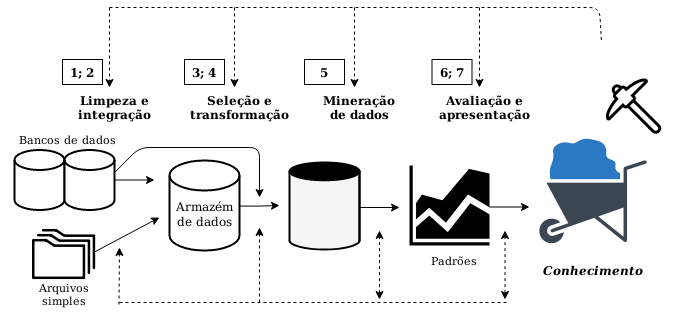
\includegraphics[width=0.85\textwidth]{img/based-on-figure-1-4-han-2011.png}
    \end{center}
    \vspace{-0.5cm}
    \legend{\ABNTEXfontereduzida \textbf{Fonte:} Figura baseada na original de \citeonline[p.~7]{Han:2011:DMC:1972541}.}
    \label{fig:diagrama-mineração-texto-han}
\end{figure}
    
    É importante notar essas 7 etapas de desenvolvimento de Mineração de Dados para abordamos a definição de MT, pois esta deriva muitas técnicas desenvolvidas na pesquisa do campo de Mineração de Dados para seu campo de aplicação, logo sistemas baseados em ambas áreas vão apresentar similaridades arquiteturais \cite[p.~1]{Feldman:2006:TMH:1076381}. 
    
    % Text mining can be broadly defined as a knowledge-intensive process in which a user interacts with a document collection over time by using a suite of analysis tools. In a manner analogous to data mining, text mining seeks to extract useful information from data sources through the identification and exploration of interesting patterns.
    
    % Because data mining assumes that data have already been stored in a structured format, much of its preprocessing focus falls on two critical tasks: Scrubbing and normalizing data and creating extensive numbers of table joins. In contrast, for text mining systems, preprocessing operations center on the identification and extraction of representative features for natural language documents. These preprocessing operations are responsible for transforming unstructured data stored in document collections into a more explicitly structured intermediate format, which is a concern that is not relevant for most data mining systems.
    
    A Mineração de Dados assume que os dados, que vão ser tratados durante seu processo, já foram armazenados em um formato estruturado, logo a maior parte de seu pré-processamento vai estar ligado às etapas 1 e 2 do processo de KDD citado, as de limpeza e integração dos dados \cite[p.~1]{Feldman:2006:TMH:1076381}. % Talvez seja necessário ao falar de linguagem natural dar um exemplo e um contra exemplo? Português e Java?
    Já na MT, como os dados de trabalho são textos, sendo texto configurado como dados desestruturados que consistem de \textit{strings} (palavras) organizadas de forma coerente e sendo pertencentes a uma linguagem natural \cite[p.~1]{Jo2018TMCIBDC}, temos que as operações de pré-processamento vão estar mais focadas em etapas adicionais, prévias às citadas para o processo de KDD, sendo estas novas direcionadas à identificação e extração de \textit{features} (atributos) representativas para documentos escritos em linguagem natural, transformando os dados não estruturados, que estão armazenados em coleções de documentos, em um formato mais explicitamente estruturado \cite[p.~1]{Feldman:2006:TMH:1076381}.
    % Text is defined as the unstructured data which consists of strings which are called words [82]
    
    % Na década de 70 houve o surgimento de diversas técnicas de gerenciamento de banco de dados, como por exemplo a 
    
    % -- Utiliza de várias áreas, falar delas
    % -- Utiliza das técnicas de RI para indexar os textos em algumas de suas aplicações
    % Text mining preprocessing operations include a variety of different types of techniques culled and adapted from information retrieval, information extraction, and computational linguistics research that transform raw, unstructured, original-format content (like that which can be downloaded from PubMed) into a carefully structured, intermediate data format. Knowledge discovery operations, in turn, are operated against this specially structured intermediate representation of the original document collection.
    
    As operações de pré-processamento para MT utilizam de várias técnicas adaptadas dos campos de Recuperação de Informação, extração de informação e linguística computacional para transformar as coleções de documentos desestruturados em dados intermediários cuidadosamente estruturados \cite[p.~2--3]{Feldman:2006:TMH:1076381}. 
    Essa estrutura intermediária é definida por um modelo representacional dos documentos de texto composto por um conjunto de atributos, sendo sempre preferidos os modelos com menor número de variáveis significativas para a representação \cite[p.~4]{Feldman:2006:TMH:1076381}.
    
    % Ressaltar denovo o suporte que a RI dá à MT, e então apresentar a diferenciação que Jo2018 faz na tabela 1.1 pag 4, e talvez a perspectiva do usuário apresentada por Zhai2016 a qual diferencia a Recuperação de Informação como Acesso dando poder de Selecionar Informação, e Mineração de Texto como Mineração possibilitando Criar Conhecimento, ele ainda apresenta a parte da Clusterização como Organização possibilitando Adicionar Estruturas/Marcações
    
    % Pensei em aqui contextualizar um pouco sobre os diversos campos que dão suporte ao KDD (Mineração de Dados) e à MT e colocar uma imagem parecida com a do \cite{Han:2011:DMC:1972541} na página 23 para mostrar os campos que dão suporte a MT
    
    A definição dos atributos para MT busca tirar proveito dos mais variados elementos presentes em um documento escrito em linguagem natural, no entanto é necessário um cuidado pois existe um grande número de palavras, frases e outros artefatos que podem comprometer o desempenho de um sistema de Mineração de Texto ou tornar a tarefa infactível \cite[p.~4]{Feldman:2006:TMH:1076381}, por isso a necessidade de identificar os melhores atributos, que trazem mais informação sobre o texto. 
    Nesse ponto que a MT pode se auxiliar de técnicas de RI para incrementar seu grupo de atributos, sendo alguns, como por exemplo o BM25 para RI ranqueada, utilizadas em competições de identificação de perfil de autores \cite{WEREN_MESTRADO_2014,WEREN_CLEF_2014,WEREN_ARTIGO_2014}. % procurar outros!!!!!.
    
    % -- Já devo diferenciar aqui
    
    % Falta falar de:
    % * Corpus
    % * Classificação binária
    % * Outros tipos de tarefas? clusterização?
    % * Feature Engineering
    %  ---> Falar da definição mais ampla, feature selection, extraction, etc.
    % * Métricas de avaliação
    
    \subsection{Corpus} \label{subsec:Corpus}
    % Jo2018 - página 6 TEXT FORMATS
        Uma coleção de
    
    \subsection{Tarefas} \label{subsec:Tarefas}
    
    \subsection{Engenharia de Atributos} \label{subsec:Engenharia-de-Atributos}
        % Falar do sentido amplo da feature engineering, abrangindo feature extraction, creation, selection, etc.
        
        \subsubsection{Atributos comuns para documentos} \label{subsubsec:Atributos-comuns-documentos}
            % Feldman2006 apresenta esses atributos básicos nas páginas 4--7
        
    \subsection{Métricas de avaliação} \label{subsec:Métricas-de-avaliação}
    % Jo2018 - página 157 são algumas, pegar de Han2011 a parte de avaliação de modelo página 364